\section{Sejarah Python}
Bahasa pemrograman Python adalah bahasa yang dibuat oleh seorang keturunan Belanda yaitu Guido van Rossum. Sampai saat ini Python masih dikembangkan oleh \textit{Python Software Foundation}. Awalnya, pembuatan bahasa pemrograman ini adalah untuk membuat skrip bahasa tingkat tinggi pada sebuah sistem operasi yang terdistribusi Amoeba. Python telah digunakan oleh beberapa pengembang dan bahkan digunakan oleh beberapa perusahaan untuk pembuatan perangkat lunak komersial. Pemrograman bahasa python ini adalah pemrogram gratis atau \textit{freeware}, sehingga dapat dikembangkan, dan tidak ada batasan dalam penyalinannya dan mendistribusikan. 

Python dikembangkan oleh Guido van Rossum pada akhir tahun delapan puluhan dan awal tahun sembilan puluhan di National Research Institute for Mathematics and Computer Science di Belanda. Python berasal dari banyak bahasa lain, termasuk ABC, Modula-3, C, C ++, Algol-68, SmallTalk, dan shell Unix dan bahasa script lainnya.
Fitur overview terbaik adalah IT mendukung metode pemrograman fungsional dan terstruktur serta OOP. Hal ini dapat digunakan sebagai bahasa scripting atau dapat dikompilasi untuk byte-kode untuk membangun aplikasi besar. Ini memberikan tingkat yang sangat tinggi pada tipe data dinamis dan mendukung memeriksa jenis dinamis. IT mendukung pengumpulan sampah otomatis. Hal ini dapat dengan mudah diintegrasikan dengan C, C ++, COM, ActiveX, CORBA, dan Java. Hal tersebut menjadi terpopuler karena kemudahan bagi programmer yang menjadikan python pemograman terbaik pada tahun 2016.

Saat ini pengembangan Python terus dilakukan oleh sekumpulan pemrogram yang dikoordinir Guido dan Python Software Foundation. Python Software Foundation adalah sebuah organisasi non-profit yang dibentuk sebagai pemegang hak cipta intelektual Python sejak versi 2.1 dan dengan demikian mencegah Python dimiliki oleh perusahaan komersial. Saat ini distribusi Python sudah mencapai versi 2.7.14 dan versi 3.6.3. 

\section{Kadek Diva Krishna Murti}

\subsection{Sejarah Python}
Python merupakan salah satu bahasa pemrograman tingkat tinggi yang menggunakan metode pemrosesan \textit{interpreted}, dimana kode program akan diproses baris per baris secara langsung dari kode program.

Bahasa pemrograman Python dirilis pertama kali oleh Guido van Rossum di Scitchting Mathematisch Centrum (CWI) Belanda pada tahun 1991. Bahasa python terinspirasi dari bahasa pemrograman ABC. Nama python tidak berasal dari nama ular yang kita kenal. Guido merupakan penggemar grup komedi Inggris bernama Monty Python. Kemudian, ia menamakan Bahasa pemrograman ciptaannya dengan nama Python.

Pada tahun 1994, Python 1.0 dirilis, yang diikuti dengan Python 2.0 pada tahun 2000. Python 3.0 keluar pada tahun 2008. Sampai saat ini Python masih dikembangkan oleh \textit{Python Software Foundation}. Bahasa Python mendukung hampir semua sistem operasi, bahkan untuk sistem operasi Linux, hampir semua distronya sudah menyertakan Python di dalamnya.


\subsection{Instalasi Anaconda}
Berikut ini merupakan langkah-langkah cara instalasi Anaconda di windows:
\begin{enumerate}
	\item Pastikan kalian telah menginstall Python sebelumnya.
	\item Klik dua kali pada installer Anaconda. Installer anaconda bisa anda dapatkan di https://www.anaconda.com/distribution/
	\item Setelah itu akan muncul window installernya. Kemudian klik ''Next'' untuk memulai instalasi.
	\begin{figure}[H]
		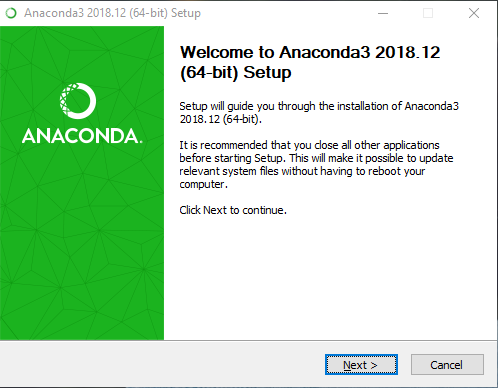
\includegraphics[width=10cm]{figures/diva/1chp1diva.png}
		\centering
	\end{figure}

	\item Baca Lisensi Agreement Anacondanya. Lalu klik ''I Agree'' jika kalian menerimanya dan untuk melajutkannya instalasinya.
	\begin{figure}[H]
		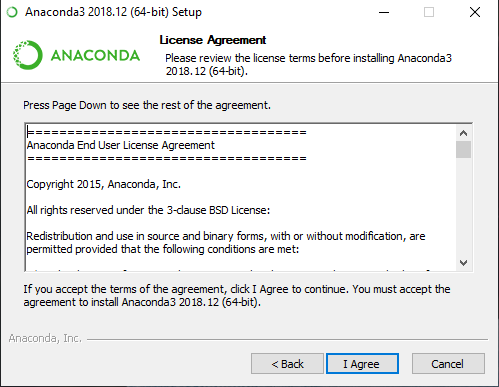
\includegraphics[width=10cm]{figures/diva/2chp1diva.png}
		\centering
	\end{figure}

	\item Selanjutnya diberi pilihan untuk menginstallnya, apakah hanya untuk kalian atau untuk semua pengguna. Disini saya memilih ''All Users'', lalu klik ''Next''.
	\begin{figure}[H]
		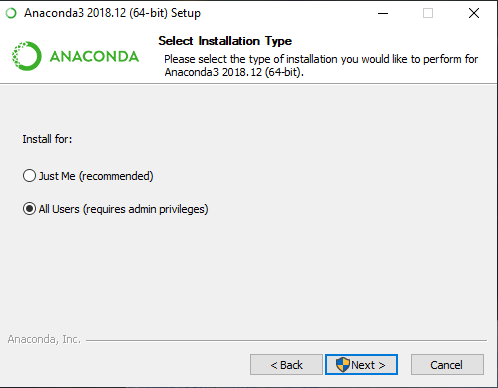
\includegraphics[width=10cm]{figures/diva/3chp1diva.png}
		\centering
	\end{figure}

	\item Kemudian pilih tujuan instalasinya. Disini saya biarkan default folder instalasinya. Setelah itu, klik ''Next''.
	\begin{figure}[H]
		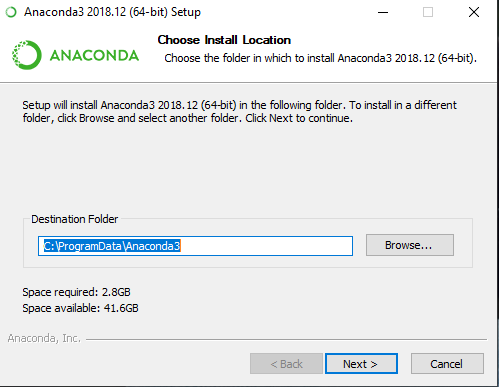
\includegraphics[width=10cm]{figures/diva/4chp1diva.png}
		\centering
	\end{figure}

	\item Setelah itu, kalian diberi beberapa opsi tambahan. Opsi pertama yaitu, ''Add Anaconda to my PATH environment variable''. Opsi ini akan menambahkan Anaconda ke PATH sistem environment variable. Opsi kedua yaitu, ''Register Anaconda as my default Python 3.7''. Opsi ini akan mendaftarkan Anaconda sebagai system Python 3.7. Saya centang kedua opsi tersebut, lalu klik ''Install''.
	\begin{figure}[H]
		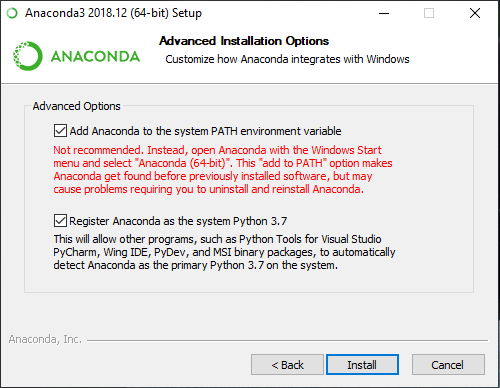
\includegraphics[width=10cm]{figures/diva/5chp1diva.png}
		\centering
	\end{figure}

	\item Tunggu hingga proses instalasi selesai.
	\begin{figure}[H]
		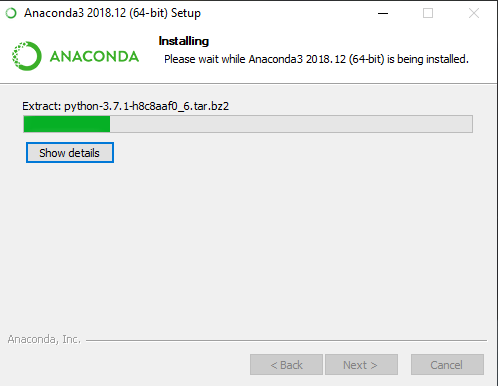
\includegraphics[width=10cm]{figures/diva/6chp1diva.png}
		\centering
	\end{figure}

	\item Kemudian klik ''Next'' untuk melanjutkan.
	\begin{figure}[H]
		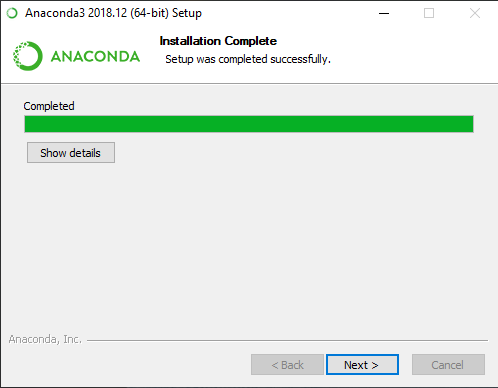
\includegraphics[width=10cm]{figures/diva/7chp1diva.png}
		\centering
	\end{figure}

	\item Selanjutnya kalian diberi pilihan untuk menginstall Microsoft VSCode. Saya klik ''Skip'' untuk melanjutkan.
	\begin{figure}[H]
		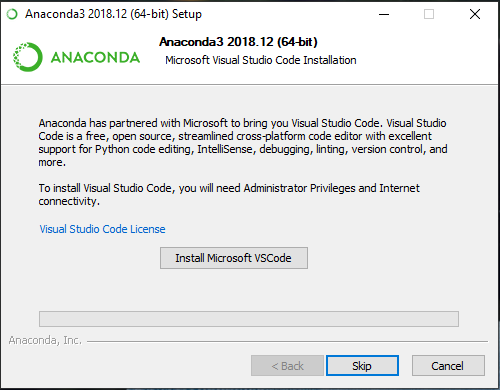
\includegraphics[width=10cm]{figures/diva/8chp1diva.png}
		\centering
	\end{figure}

	\item Kemudian klik ''Finish'' untuk selesai.
	\begin{figure}[H]
		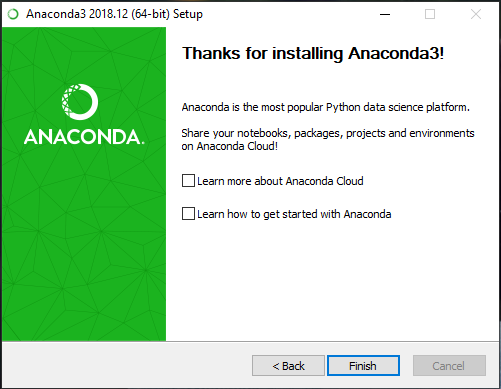
\includegraphics[width=10cm]{figures/diva/9chp1diva.png}
		\centering
	\end{figure}

	\item Untuk mengecek apakah Anaconda telah terinstall yaitu dengan cara membuka Command Prompt. Lalu ketikan ''conda -V'' dan tekan enter, kode itu akan mengecek versi Anaconda yang terinstall.
	\begin{figure}[H]
		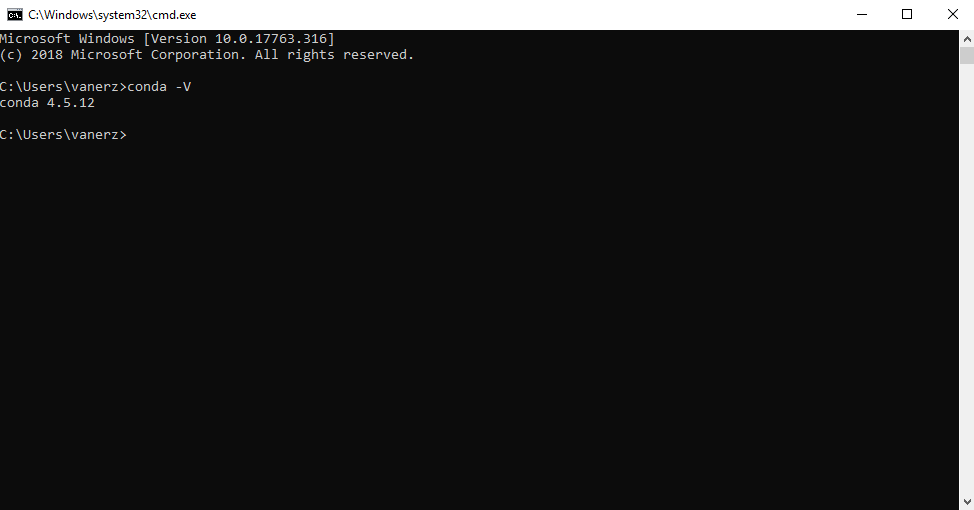
\includegraphics[width=10cm]{figures/diva/10chp1diva.png}
		\centering
	\end{figure}

\end{enumerate}

\subsection{Penggunaan Spyder}

Terdapat 2 cara menjalankan Spyder. Yang pertama dengan Anaconda Prompt dan yang kedua dengan Anaconda Navigation. Berikut ini merupakan langkah-langkah cara menjalankan Spyder di windows:

\begin{itemize}
	\item Anaconda Prompt

	\begin{enumerate}
		
		\item Pertama klik start, lalu cari ''Anaconda Prompt''.
		\begin{figure}[H]
			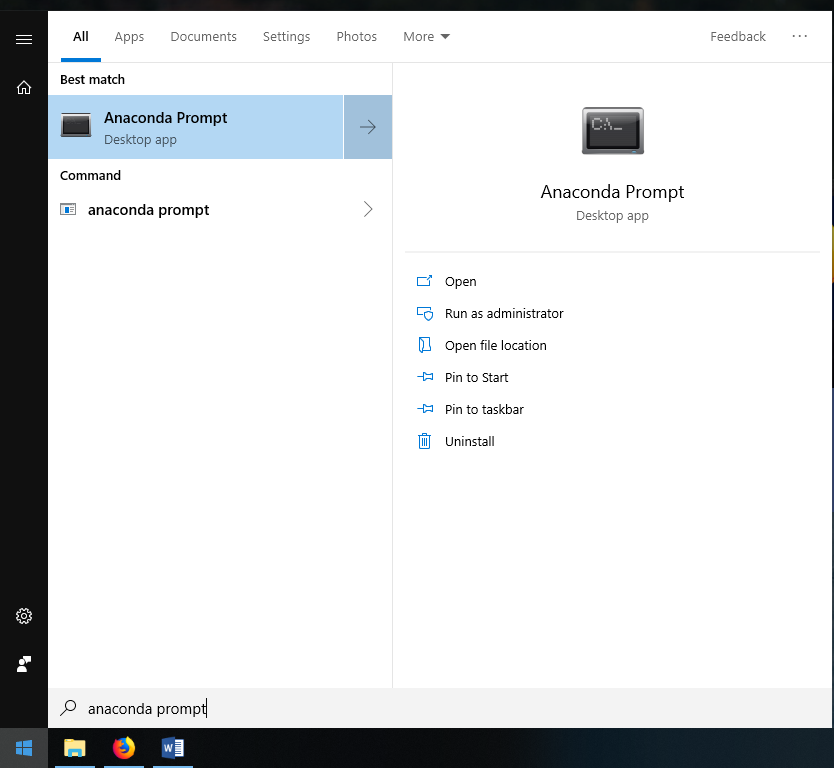
\includegraphics[width=10cm]{figures/diva/11chp1diva.png}
			\centering
		\end{figure}		
		\item Selanjutnya akan muncul sebuah prompt. Kemudian ketikan ''start spyder'' dan tekan enter.
		\begin{figure}[H]
			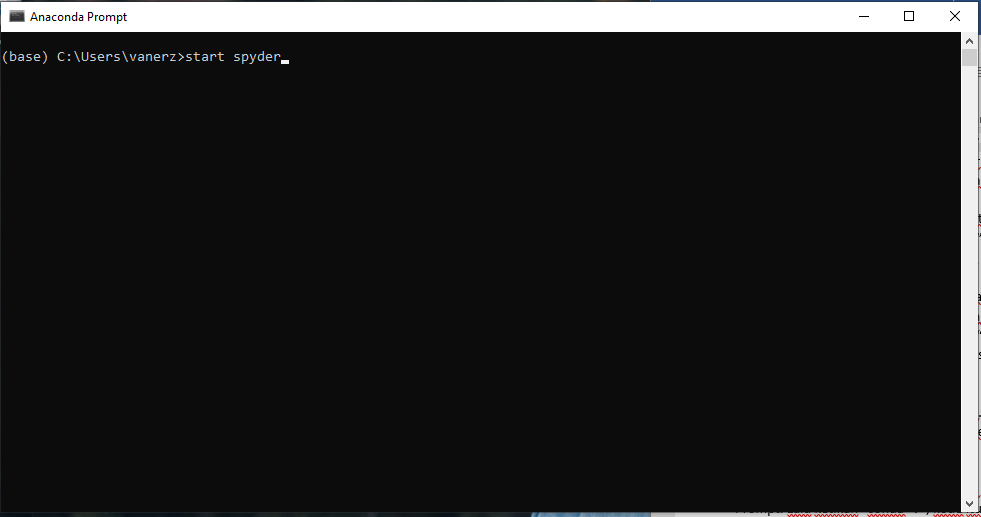
\includegraphics[width=10cm]{figures/diva/12chp1diva.png}
			\centering
		\end{figure}
		\item Lalu tunggu sampai selesai.
		\begin{figure}[H]
			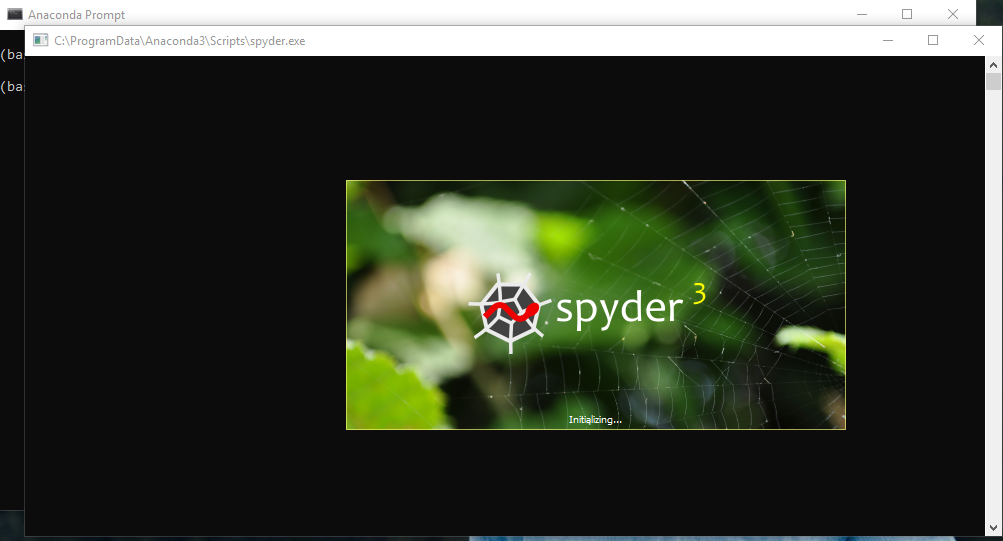
\includegraphics[width=10cm]{figures/diva/13chp1diva.png}
			\centering
		\end{figure}

	\end{enumerate}
	\item Anaconda Navigation

	\begin{enumerate}
		\item Pertama klik start, lalu cari ''Anaconda Navigation''.
		\begin{figure}[H]
			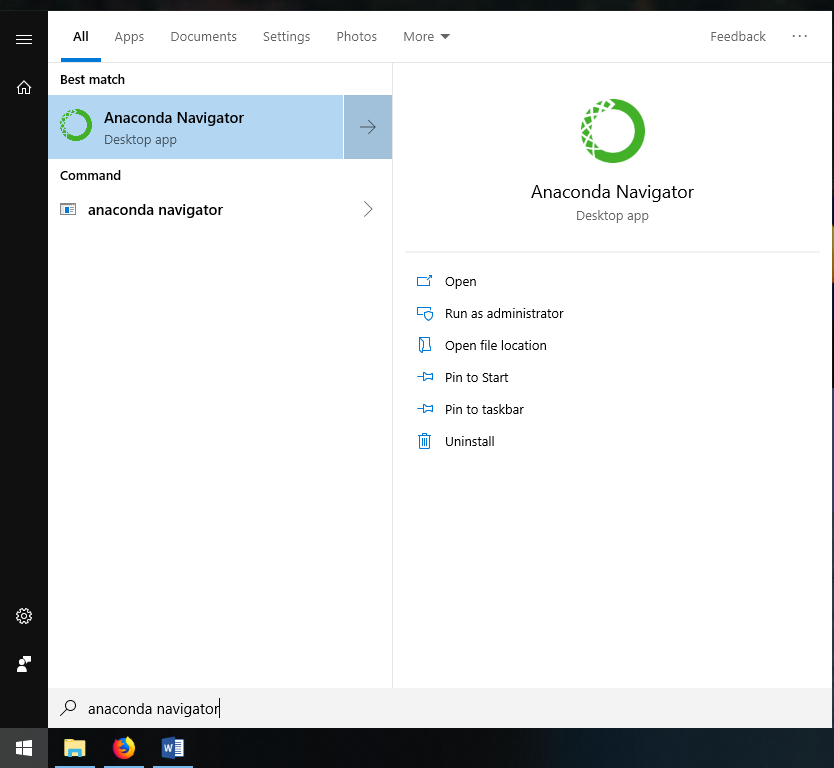
\includegraphics[width=10cm]{figures/diva/14chp1diva.png}
			\centering
		\end{figure}
		\item Selanjutnya akan muncul sebuah window. Kemudian klik ''Launch'' pada menu Spyder.
		\begin{figure}[H]
			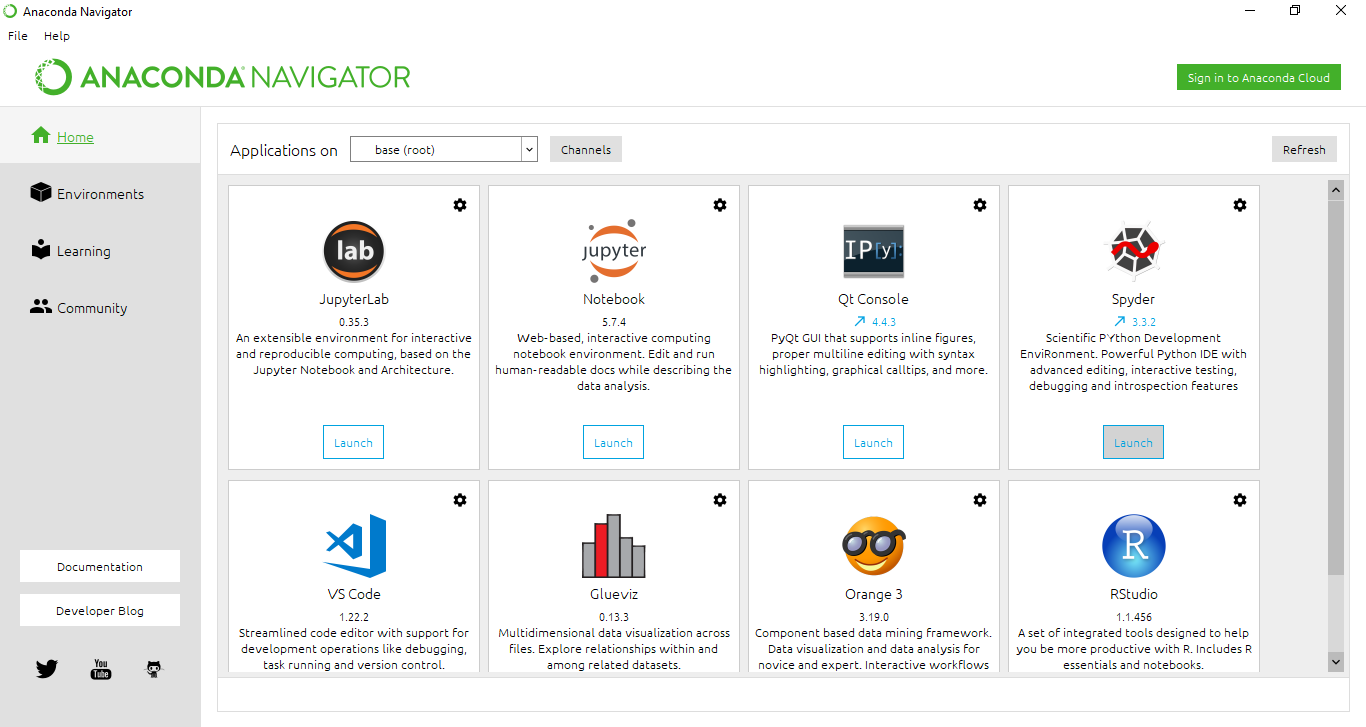
\includegraphics[width=10cm]{figures/diva/15chp1diva.png}
			\centering
		\end{figure}
		\item Lalu tunggu sampai selesai.
		\begin{figure}[H]
			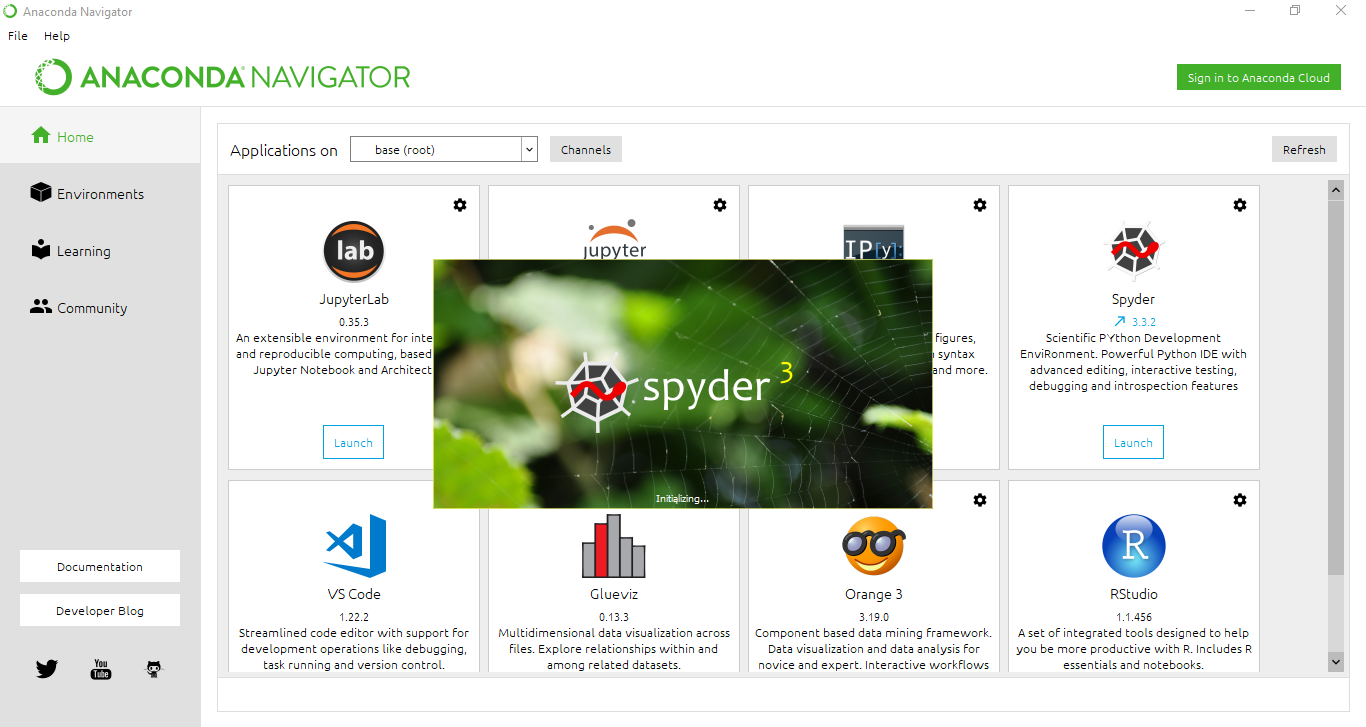
\includegraphics[width=10cm]{figures/diva/16chp1diva.png}
			\centering
		\end{figure}

	\end{enumerate}
\end{itemize}

Apabila muncul window in ketika pertama kali menjalankan Spyder, pilih “Allow Access”.
\begin{figure}[H]
	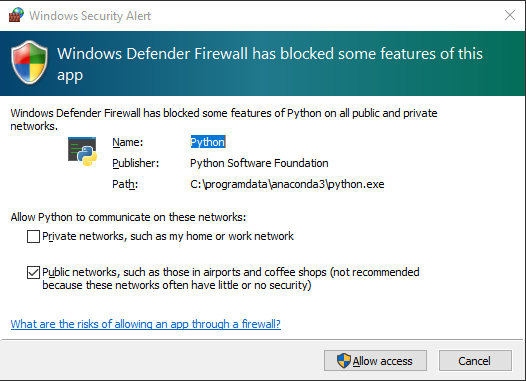
\includegraphics[width=10cm]{figures/diva/17chp1diva.png}
	\centering
\end{figure}
		
Berikut ini merupakan gambar dari Spyder
\begin{figure}[H]
	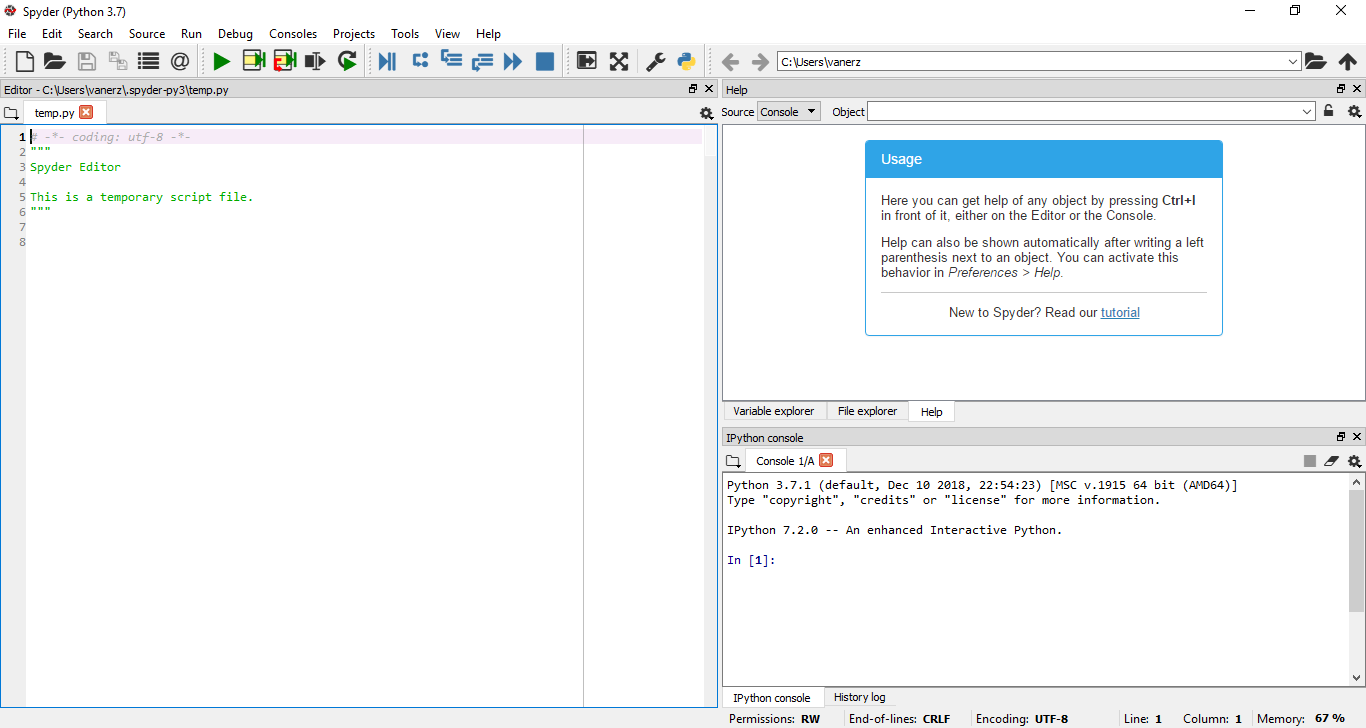
\includegraphics[width=10cm]{figures/diva/18chp1diva.png}
	\centering
\end{figure}

